\part{Soluções Apresentadas}
\chapter[Introdução]{Introdução}
Neste capítulo abordaremos todas as soluções idealizadas para o projeto. O capítulo está dividido conforme os grupos descritos na subseção ~\ref{subsec:divisao}.

\chapter[Estruturas e Materiais]{Estruturas e Materiais}

\chapter[Smart Grid]{Smart Grid}

\begin{table}[h]
  \centering
  \caption{Energia Eólica - Vantagens x Desvantagens}
  \label{my-label}
  \begin{tabular}{|l|l|}
    \hline
    \multicolumn{2}{|c|}{\textbf{Energia Eólica}}                                         \\ \hline
    \multicolumn{1}{|c|}{\textbf{Vantagens}} & \multicolumn{1}{c|}{\textbf{Desvantagens}} \\ \hline
    Energia Sustentável                      & Alto Custo                                 \\ \hline
    Energia Limpa                            & Baixa velocidade do vento na região        \\ \hline
    Energia Renovável                        & Pouca Área para instalação dos equipamento \\ \hline
  \end{tabular}
\end{table}

\begin{table}[h]
  \centering
  \caption{Energia Solar Fotovoltaica - Vantagens x Desvantagens}
  \label{my-label}
  \begin{tabular}{|l|c|}
    \hline
    \multicolumn{2}{|c|}{\textbf{Energia Solar Fotovoltaica}}                                                \\ \hline
    \multicolumn{1}{|c|}{\textbf{Vantagens}}             & \textbf{Desvantagens}                             \\ \hline
    Energia Sustentável                                  & \multicolumn{1}{l|}{Alto custo financeiro}        \\ \hline
    Energia limpa                                        & \multicolumn{1}{l|}{Geração apenas durante o dia} \\ \hline
    Simples manutenção                                   & -                                                 \\ \hline
    Alta incidência solar na região                      & -                                                 \\ \hline
    Vida útil dos painéis longa                          & -                                                 \\ \hline
    Tempo de retorno do investimento em cerca de 10 anos & -                                                 \\ \hline
  \end{tabular}
\end{table}


\begin{table}[h]
  \centering
  \caption{Gerador Movido a Biodiesel - Vantagens x Desvantagens}
  \label{my-label}
  \begin{tabular}{|c|l|}
    \hline
    \multicolumn{2}{|c|}{\textbf{Gerador Movido a Biodiesel}}                                            \\ \hline
    \textbf{Vantagens}                                      & \multicolumn{1}{c|}{\textbf{Desvantagens}} \\ \hline
    \multicolumn{1}{|l|}{Energia Sustentável}               & Alto consumo de biodiesel                  \\ \hline
    \multicolumn{1}{|l|}{Biocombustível produzido pela FGA} & Rendimento baixo                           \\ \hline
    -                                                       & Alto custo financeiro                      \\ \hline
    -                                                       & Manutenção periódica                       \\ \hline
  \end{tabular}
\end{table}


\chapter[Controle de Acesso]{Controle de Acesso}
\section{Escolha da Tecnologia}
A área de Controle de Acesso está aqui subdividida em três grandes principais frentes tecnológicas.
São elas: controle da entrada do estacionamento privativo, controle da entrada em salas e laboratórios
e, por fim, controle de frequência durante as aulas.

Dentre essas frentes, foram elegidas três possibilidades diferentes para a inserção na Universidade.
A tabela a seguir elicita-as, bem como apresenta as vantagens e desvantagens para cada um dos casos.

\begin{table}[h]
  \centering
  \caption{Tecnologias de Controle de Acesso - Vantagens x Desvantagens}
  \label{my-label}
  \begin{tabular}{|l|l|l|}
    \hline
    \multicolumn{1}{|c|}{\textbf{Tecnologia}} & \multicolumn{1}{c|}{\textbf{Vantagens}}                                                                         & \multicolumn{1}{c|}{\textbf{Desvantagens}}                                                                                                            \\ \hline
    Leitor biométrico                         & \begin{tabular}[c]{@{}l@{}}- Difícil de burlar \\ - Confiável\end{tabular}                                      & \begin{tabular}[c]{@{}l@{}}- Pode gerar falhas na leitura \\ - Não reconhecer uma \\ digital cadastrada\\ - Sistema caro\\ - Sistema frágil\end{tabular} \\ \hline
    Leitor facial/ Leitor de íris             & \begin{tabular}[c]{@{}l@{}}- Difícil de burlar \\ - Confiável\end{tabular}                                      & \begin{tabular}[c]{@{}l@{}}- Sistema de implementação\\ cara\\ - Demora para análise de \\cada pessoa\\ - Risco de furto\\ - Frágil\end{tabular}          \\ \hline
    Leitor RFID                               & \begin{tabular}[c]{@{}l@{}}- Fácil de utilizar\\ - Difícil de burlar\\ - Único para cada estudante\end{tabular} & \begin{tabular}[c]{@{}l@{}}- Custo extra para a \\faculdade\\ - Risco de perda do \\documento\end{tabular}                                                \\ \hline
  \end{tabular}
\end{table}

Apesar de todas as tecnologias sugeridas apresentarem vantagens e desvantagens, o sistema RFID foi o escolhido para atender
a demanda. Esta escolha se deu em virtude deste ser mais eficaz, eficiente e mais acessível financeiramente em relação aos
outros.

\subsection{Breve Descrição da Tecnologia RFID}
O sistema funciona RFID (do inglês \textit{Radio-Frequency IDentification}) é um tecnologia que permite identificação automática
 através de sinais de rádio. Neste projeto será implementado de  por meio de um chip dentro de um cartão, armazenando o
 nome e matrícula do aluno dono do documento e sempre que o documento for apresentado, seus dados serão apresentados nos
 display dos equipamentos. Levando em conta que tanto alunos como professores serão portadores deste documento com chip,
 para o alunos o cartão será utilizado como carteirinha, e para os professores como crachá.

Apesar de todo o grupo de controle de acesso utilizar esta ferramenta, cada uma das frentes utiliza o sistema de forma
diferente e com aparelhos diferentes. Desta forma, cada área tem suas particularidades de funcionamento e regras, como será
 mostrado e explicado a seguir.

\section{Controle de Frequência}
Para o controle de frequência nas aulas, será utilizado o seguinte aparelho (apresentado anteriormente no Ponto de Controle 1).
O funcionamento dele acontece independente de sinal de WiFi e o aparelho é de porte único do professor.

\begin{figure}[!h]
  \centering
  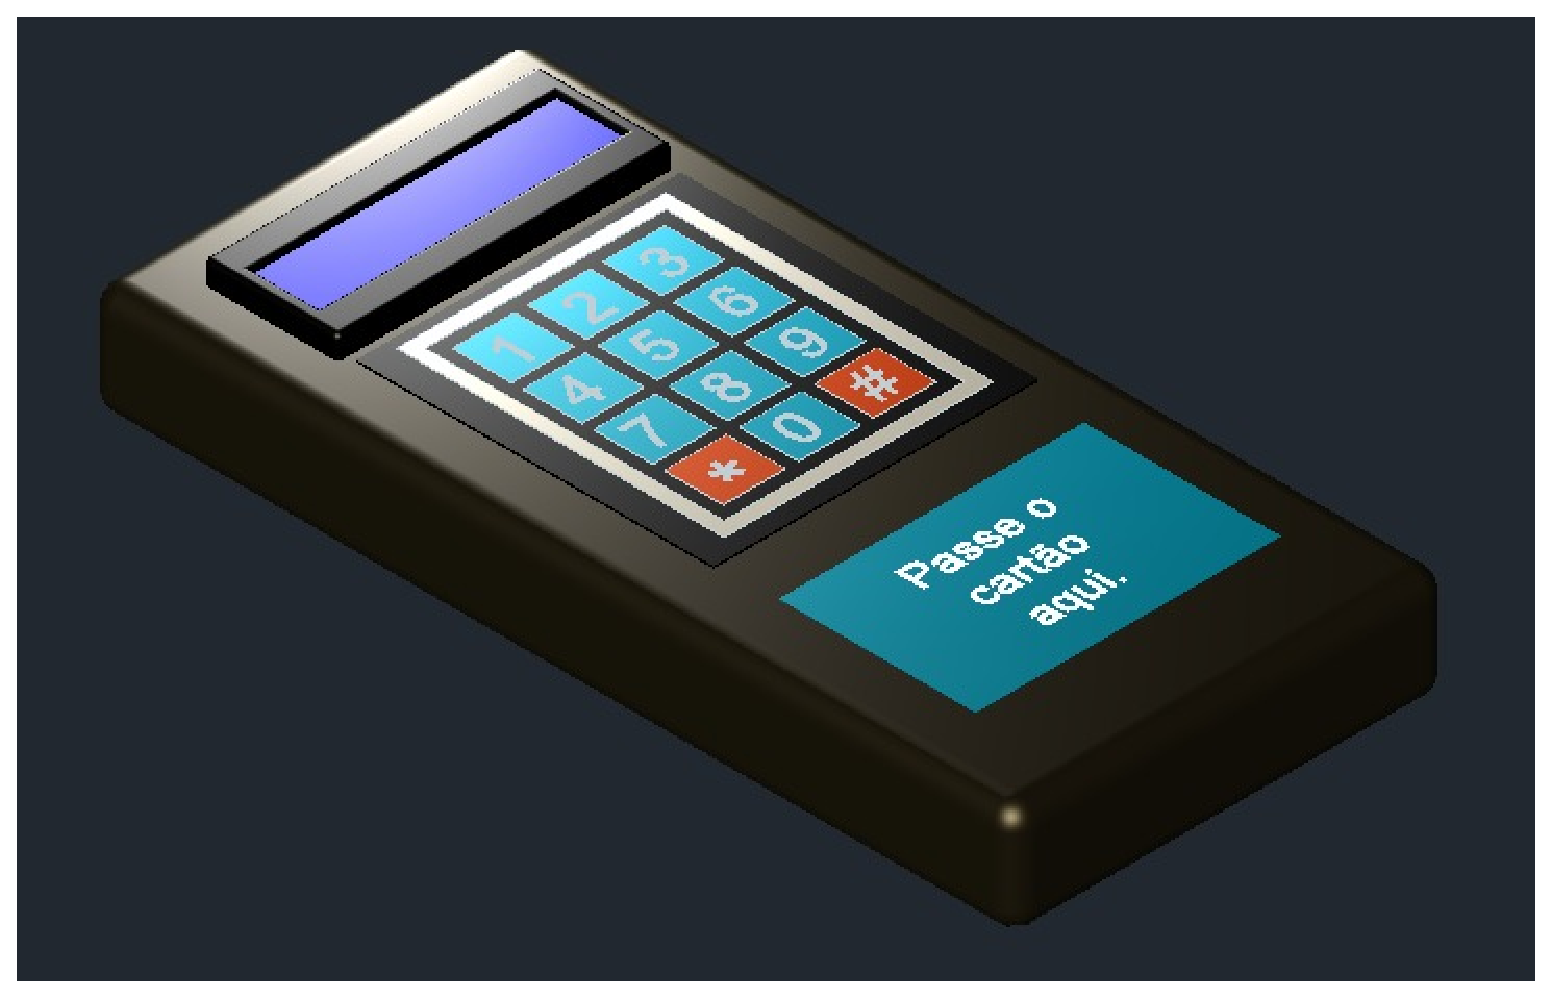
\includegraphics[keepaspectratio=true,scale=0.45]{figuras/freq.eps}
  \caption{Aparelho Para Controle de Frequência}
\end{figure}

Em relação à aspectos técnicos do aparelho, a figura a seguir mostra detalhadamente quais os instrumentos utilizados.

\begin{figure}[h]
  \centering
  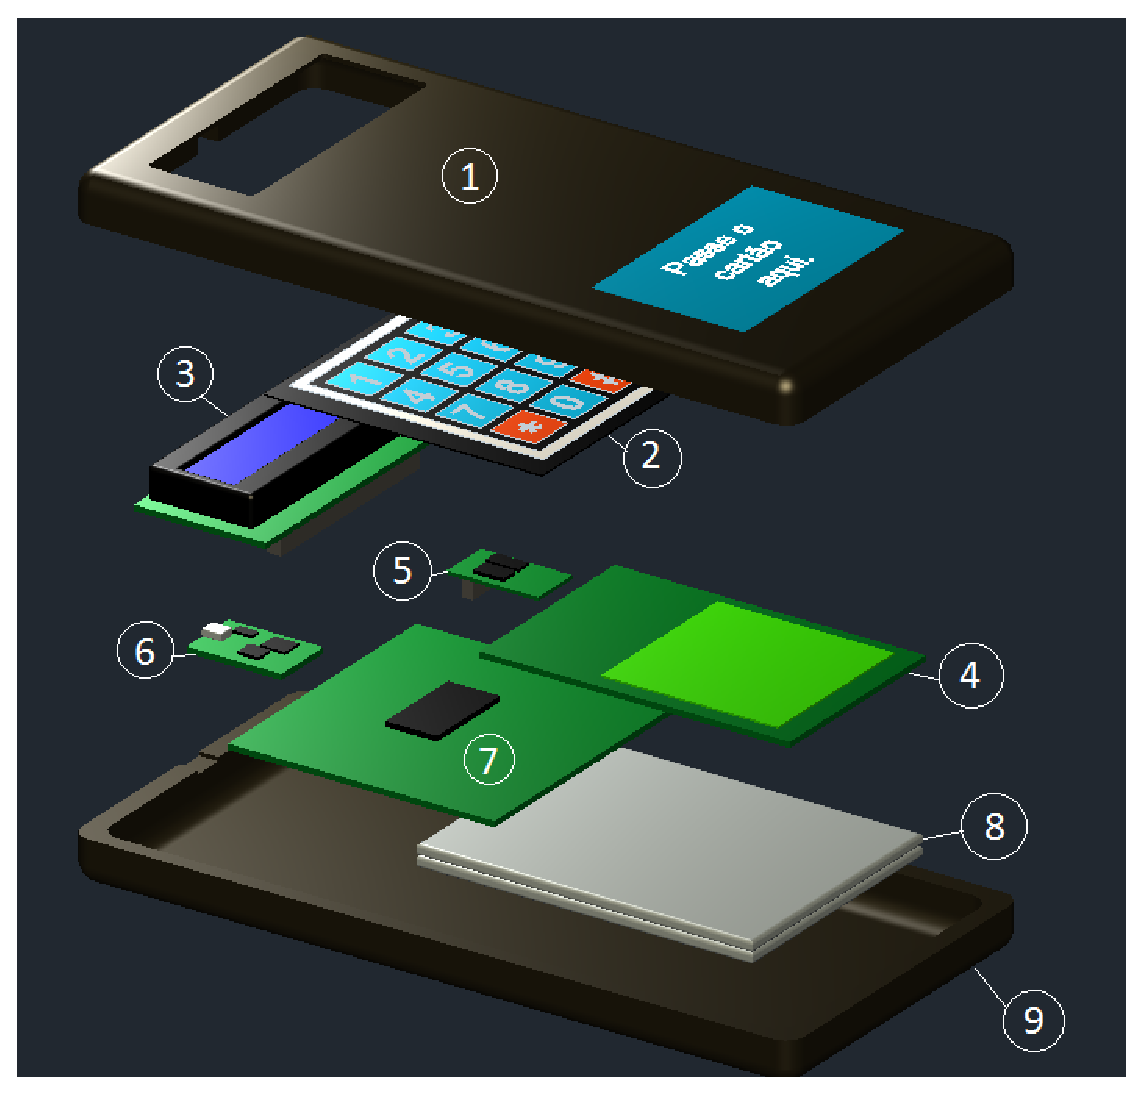
\includegraphics[keepaspectratio=true,scale=0.45]{figuras/aberto.eps}
  \caption{Aparelho Para Controle de Frequência Detalhado}
\end{figure}

Cada um dos componentes possui sua função individual:
\begin{itemize}
  \item Componentes 1 e 9: Case superior e inferior. Há um orifício na parte superior do dispositivo para passagem do conector USB.
  \item Componente 2: Teclado matricial de película 12 teclas.
  \item Componente 3: Display LCD 16x2 com backlight
  \item Componente 4: módulo Leitor de cartões RFID Mfrc522 Mifare, faz leitura e escrita em cartões RFID.
  \item Componente 5: Módulo WiFi ESP8266 ESP-01, se conecta com a rede wifi e transmite e recebe dados servidor online.
  \item Componente 6: Módulo Carregador de Baterias de Lítio TP4056, carrega a bateria através do seu conector USB.
  \item Componente 7: Placa controladora faz as conexões com os demais componentes e possui um microcontrolador ATmega1280 16au da família AVR com o bootloader do Arduino mega.
  \item Componente 8: Baterias do tablet Dl Lenoxx Navcity Phaser. Possuem capacidade de 2000mAh e tensão de 3,7v.
\end{itemize}

Cada um desses microcomponentes têm funções específicas que garantem o funcionamento adequado do instrumento. Sob uma ótica mais específica temos:

\subsection{Kit Módulo Leitor Rfid Mfrc522 Mifare}


Este módulo leitor RFID baseado no chip MFRC522 da empresa NXP é altamente utilizado em comunicação sem contato a uma frequência de 13,56MHz. Este chip, de baixo consumo e pequeno tamanho, permite sem contato ler e escrever em cartões que seguem o padrão Mifare, muito usado no mercado.

Este leitor RFID possui as ferramentas para um projeto de controle de acesso ou sistemas de segurança a um ótimo preço.

Este componentes vai ser conectado a o microcontrolador através dos pinos especiais sda(pino 44), sck(pino 20), miso(pino 22) e mosi(pino 21).

\begin{figure}[!h]
  \centering
  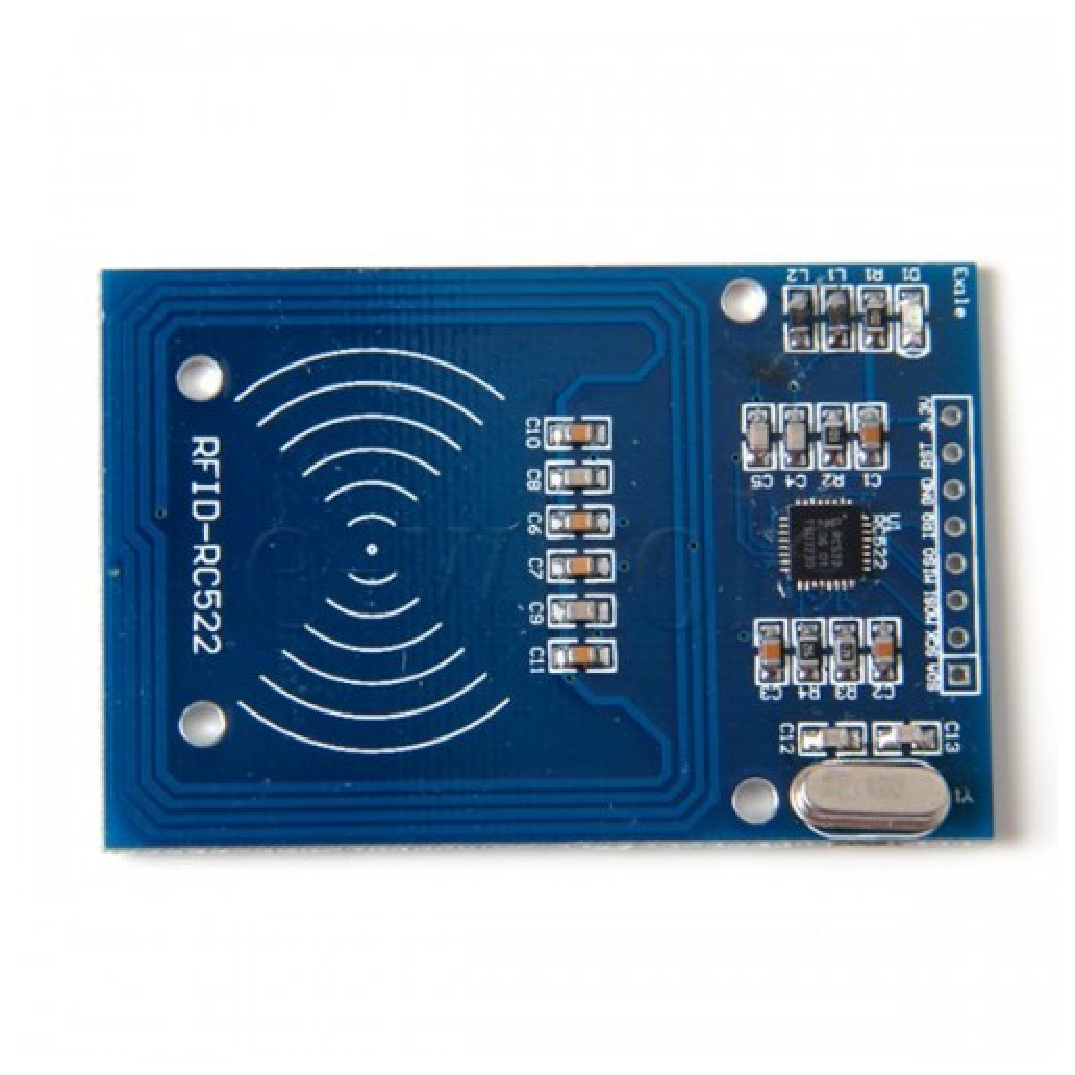
\includegraphics[keepaspectratio=true,scale=0.5]{figuras/rfid.eps}
  \caption{Módulo Leitor Rfid Mfrc522 Mifare}
\end{figure}


\subsection{Módulo WiFi ESP8266 ESP-01}
O módulo wireless ESP8266 foi desenvolvido para que seja possível conectar o microcontrolador a uma conexão WiFi de forma fácil, eficaz e a um baixo preço.

Este módulo suporta as redes 802.11 b/g/n, muito usadas atualmente, podendo trabalhar como um Ponto de Acesso (Access Point) ou como uma Estação (Station), enviando e recebendo dados.

A comunicação serial pelo protocolo RS-232, irá utilizar as portas RX(pino 45) e TX(pino 46) do microcontrolador que possuem suporte para este protocolo de comunicação TX e diretamente a protoboard. Ele será utilizado para enviar as informações coletadas pelo dispositivo ao banco de dados na rede.
\pagebreak

\begin{figure}[!h]
  \centering
  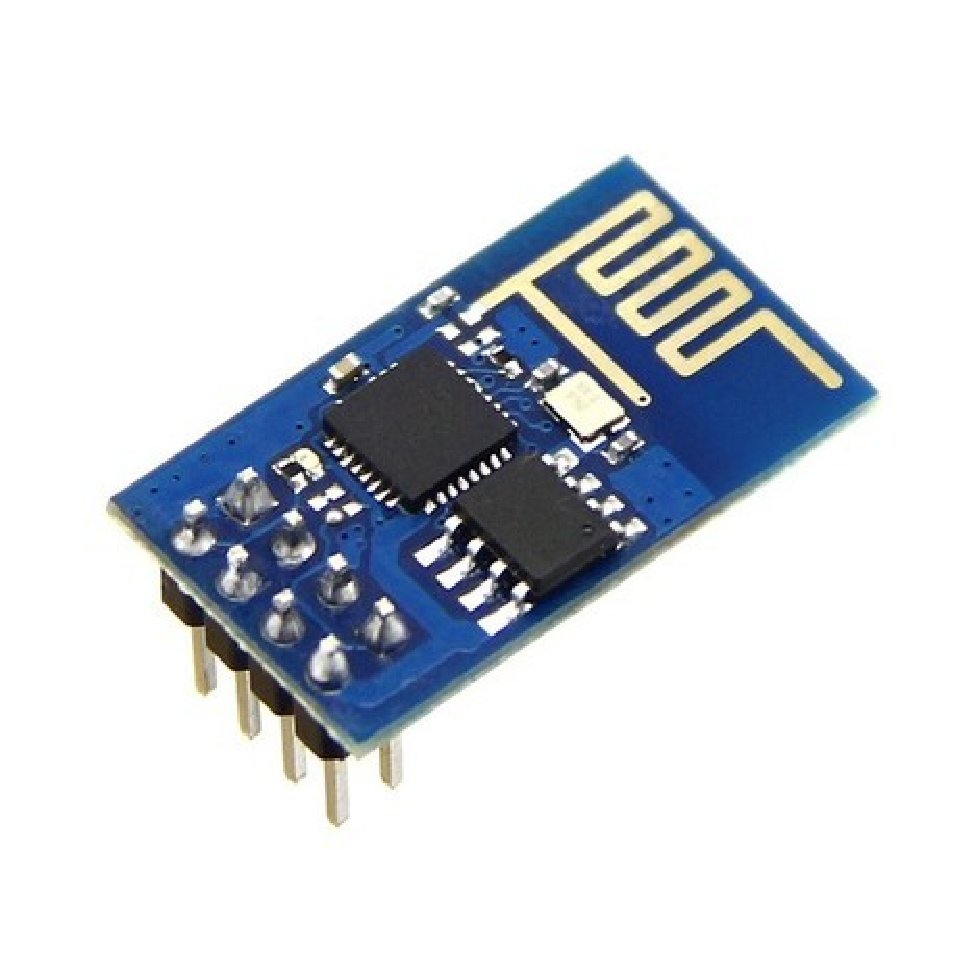
\includegraphics[keepaspectratio=true,scale=0.5]{figuras/wifi.eps}
  \caption{Módulo Leitor Rfid Mfrc522 Mifare}
\end{figure}


\subsection{Display LCD 16x2}
Este é um display LCD de 16 colunas por 2 linhas, backlight azul e escrita branca. Possui o controlador HD44780 usado em toda indústria de LCD's como base de interface.

A interface com microcontrolador é muito simples, sendo basicamente 4 pinos digitais de dados e 2 pinos digitais de controle. Confira no link o Datasheet Display LCD 16x2. O display será utilizado para mostrar a matrícula e o nome do dono da carteirinha, possibilitar ao professor selecionar a disciplina que deseja passar a chamada e outras informações que forem necessárias.

\begin{figure}[!h]
  \centering
  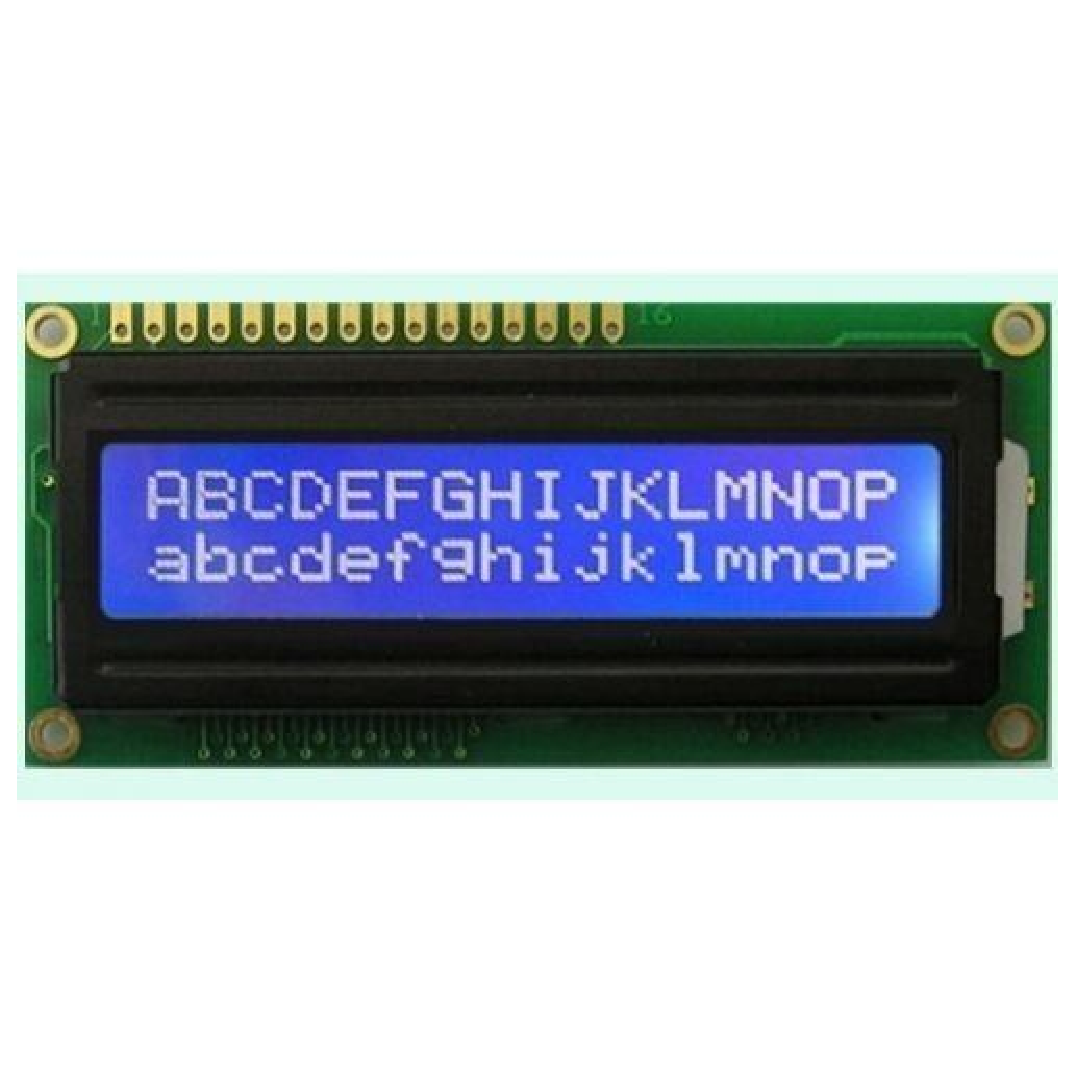
\includegraphics[keepaspectratio=true,scale=0.45]{figuras/lcd.eps}
  \caption{Display LCD}
\end{figure}

\pagebreak

\subsection{Teclado de Película 4x4}
O Teclado Matricial 4x4 é um componente utilizado para entrada de dados. Ele possui 16 teclas dispostas em 4 linhas x 4 colunas, e um conector de 8 pinos para ligação. Ele necessita de 8 pinos digitais para funcionar, sendo 4 configurados como saída(OUTPUT) e 4 como leitura(INPUT). Os pinos de saída são acionados como um contador em anel, elevando um pinos em nível alto e os demais em nível baixo, após um tempo determinado outro pino fica em nível alto e o resto em nível baixo e o ciclo se repete para cada pino. Cada pino é conectado em uma coluna da matriz e os pinos de leitura lêem as quatro linhas individualmente. Desta forma quando um botão é pressionado,  é possível determinar a linha e coluna da matriz.

\begin{figure}[!h]
  \centering
  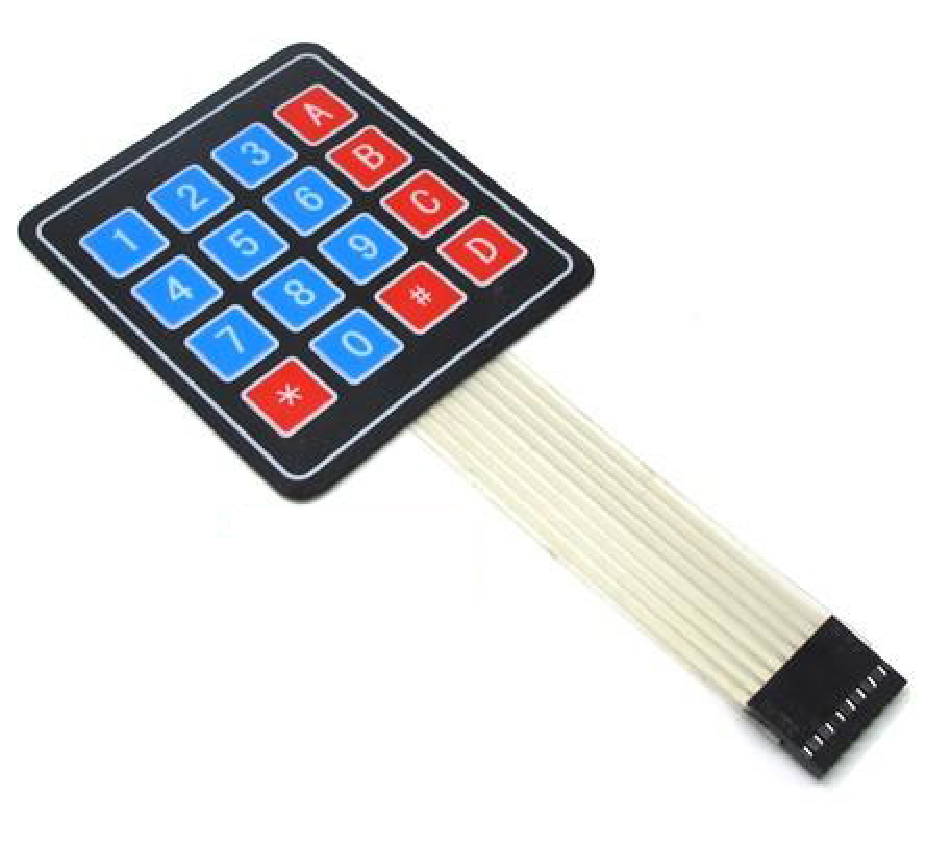
\includegraphics[keepaspectratio=true,scale=0.45]{figuras/teclado.eps}
  \caption{Teclado de Película 4x4}
\end{figure}

\subsection{Carregador de Bateria Lipo - Mini Usb TP4056}
Módulo carregador de baterias TP4056 para baterias de lítio, possibilita que as baterias sejam recarregadas sem a necessidade de removê-las do circuito. Módulo se conecta diretamente com a bateria e carrega a mesma quando é conectado um carregador USB. A corrente é cortada quando detecta que a carga está completa e possui um led indicador de carregamento. Contudo para aferir o nível de carga da bateria, será utilizado um pino analógico do microcontrolador. Medindo o nível de tensão na bateria será possível  informar o  nível de  carga através do display LCD, o que é mais prático.


\begin{figure}[!h]
  \centering
  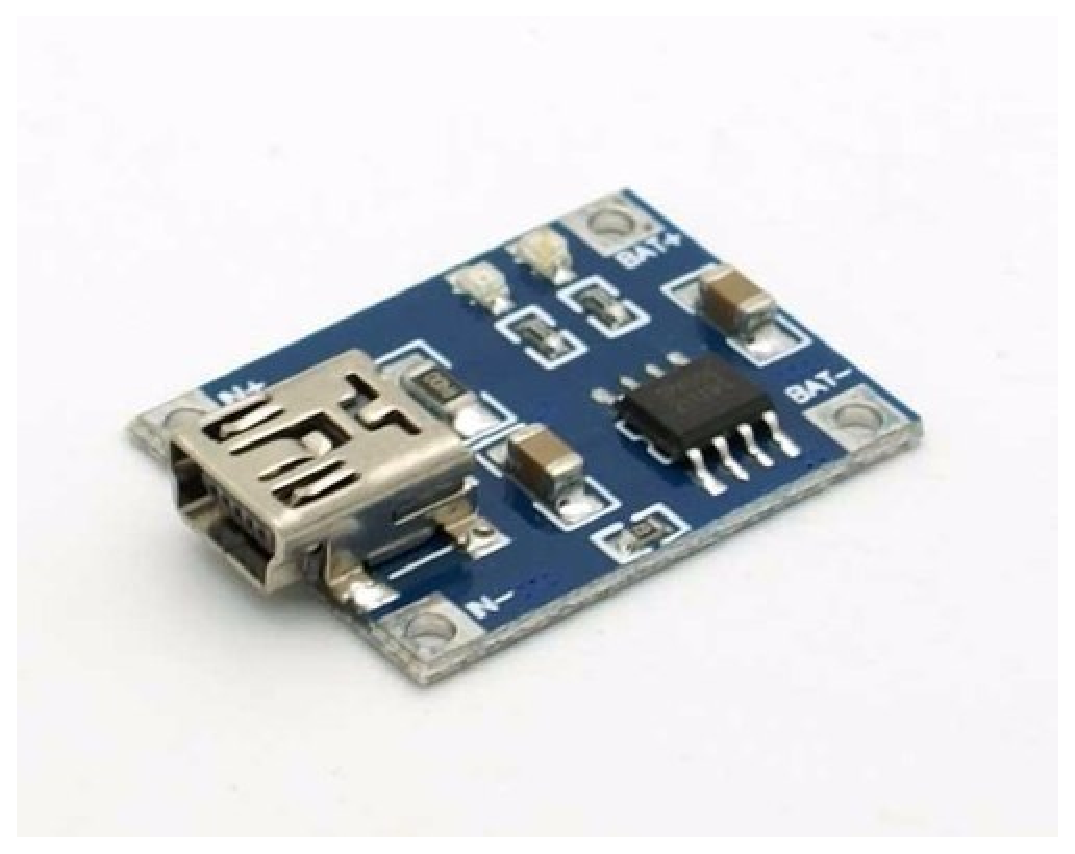
\includegraphics[keepaspectratio=true,scale=0.45]{figuras/carregador.eps}
  \caption{Carregador de Bateria Lipo}
\end{figure}

\subsection{Bateria}
Serão utilizadas duas baterias 3.7V 2000mAh em série para alimentar o dispositivo. A tensão fornecida será 7.4~6V e uma autonomia de cerca de 8 horas em uso á 157 horas (cerca de 6 dias) em \textit{standby}. Todos os componentes têm uma tensão de operação de 3.3V, apenas o display LCD opera com 5V. Para regular a tensão, será utilizado CI regulador de tensão 7805 para o display e o LM1117T para os demais.

\begin{figure}[!h]
  \centering
  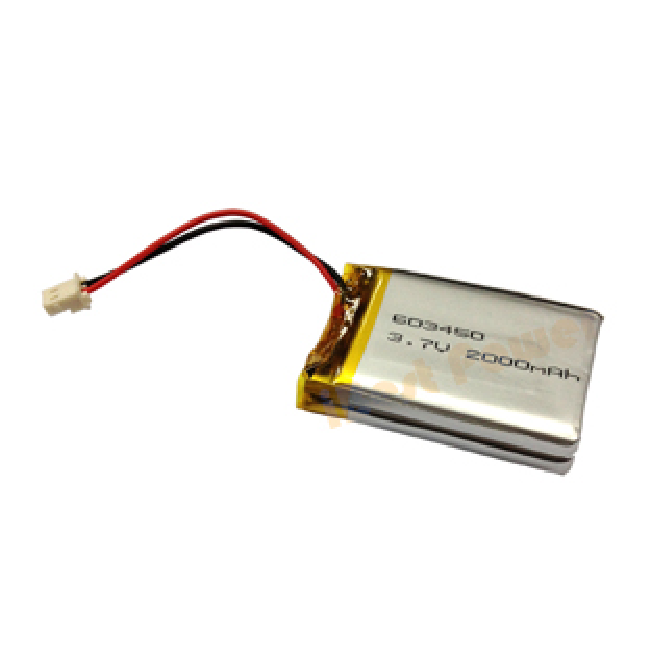
\includegraphics[keepaspectratio=true,scale=0.7]{figuras/bateria.eps}
  \caption{Bateria 2000mAh}
\end{figure}

\subsection{Microcontrolador ATmega1280}
O microcontrolador escolhido foi o ATmega1280 em função de ser o microcontrolador presente no Arduino Mega e seu número de pinos. Por isso, será possível utilizar o bootloader do arduino no microcontrolador, facilitando a programação uma vez que todos os componentes utilizados no projeto possuem bibliotecas que facilitam seu uso e implementação para arduino. Seu número de pinos digitais e especiais (TX, RX, MOSI, MISO, SDA, SCK) também foi levado em consideração durante o processo de escolha.

Em seguida, foram testados e pesquisados dados de tensão, autonomia e corrente, devido ser um aparelho portátil e de funcionamento independente da internet e sem estar ligado na tomada. Todos os dados estão apresentados na tabela a seguir.

\begin{table}[!h]
  \centering
  \caption{Dados dos Componentes - Aparelho de Frequência}
  \begin{tabular}{|l|c|c|c|}
    \hline
    \multicolumn{1}{|c|}{\textbf{Componentes}}                  & \parbox[t]{2cm}{\textbf{Corrente máxima (mA)}} & \multicolumn{1}{l|}{\parbox[t]{2cm}{\textbf{Corrente mínima (mA)}}} & \parbox[t]{5cm}{\textbf{Tensão de nominal (V)}} \\ \hline
    \parbox[t]{6cm}{Kit Módulo Leitor Rfid Mfrc522 Mifare\\}                       & 13                            & 10                                        & 3,3                            \\ \hline
    \parbox[t]{6cm}{Cartão RFID Programável Mifare 13,56Mhz}                     & -                             & -                                         & -                              \\ \hline
    Módulo WiFi ESP8266 ESP-01                                  & 215                           & 0,9                                       & 3,3                            \\ \hline
    LCD 16x2                                                    & 1,5                           & 1                                         & 5                              \\ \hline
    Teclado de película 4x3                                     & 0,3                           & 0,3                                       & 3,3                            \\ \hline
    ATmega1280                                                  & 20                            & 0,5                                       & 1,8                     \\ \hline
    \parbox[t]{6cm}{Carregador De Bateria   Lipo - Mini Usb Tp4056}                & 0                             & 0                                         & 5                              \\ \hline
    Bateria 3,7v 2000mah                                        & 0                             & 0                                         & 3,7                            \\ \hline
    \multicolumn{1}{|c|}{\textbf{TOTAL}}                        & 249,8                         & 12,7                                      & -                              \\ \hline
  \multicolumn{1}{|c|}{\parbox[t]{5cm}{\textbf{Autonomia da bateria (Horas)}}} & 8                             & 157                                       & -                              \\ \hline
  \end{tabular}
\end{table}

Com base nos dados da tabela anterior, pode-se afirmar que a autonomia da bateria do dispositivo em uso contínuo poderá ser de até 8 horas e, em standby, até 6 dias. Dado que o dispositivo poderá entrar em um modo de dormência, desabilitando o wifi, o leitor e até o próprio microcontrolador, ele poderá ter uma autonomia maior que 8 horas se entrar de forma automática neste modo enquanto aguarda uso.

Por fim, em termos econômicos, obtivemos o seguintes dados de custos:


\begin{table}[!h]
  \centering
  \caption{Custos dos Componentes - Aparelho de Frequência}
  \label{my-label}
    \begin{tabular}{|l|c|c|}
    \hline
    \multicolumn{1}{|c|}{\textbf{Componente}}    & \textbf{Custo} & \textbf{Fonte}                                                                                                \\ \hline
    \parbox[t]{7cm}{Kit Módulo Leitor Rfid Mfrc522 Mifare}        & R\$ 39,90      & \href{http://www.filipeflop.com/pd-6b883-kit-modulo-leitor-rfid-mfrc522-mifare.html}{Fonte 1}                                 \\ \hline
    \parbox[t]{7cm}{Cartão RFID Programável Mifare 13,56Mhz}      & R\$ 5,90       & \href{http://www.filipeflop.com/pd-1c240a-cartao-rfid-programavel-mifare-13-56mhz.html}{Fonte 2}                              \\ \hline
    Módulo WiFi ESP8266 ESP-01                   & R\$ 29,90      & \href{http://www.filipeflop.com/pd-1f55ad-modulo-wifi-esp8266-esp-01.html}{Fonte 3}                                           \\ \hline
    LCD 16x2                                     & R\$ 16,90      & \href{http://www.filipeflop.com/pd-6b7e4-display-lcd-16x2.html?ct=\&p=1\&s=1}{Fonte 4}                                        \\ \hline
    Teclado de película 4x3                      & R\$ 10,90      & \href{http://www.filipeflop.com/pd-218a98-teclado-matricial-de-membrana-12-teclas.html?ct=\&p=1\&s=1}{Fonte 5}                \\ \hline
    ATmega1280                                   & R\$ 60,00      & \href{http://produto.mercadolivre.com.br/MLB-831270785-lote-5-pecas-atmega1280-16au-marca-atmel-100-tqfp-atmel-\_JM}{Fonte 6} \\ \hline
    \parbox[t]{7cm}{Carregador De Bateria Lipo - Mini Usb Tp4056} & R\$ 9,90       & \href{http://www.filipeflop.com/pd-36ef09-modulo-carregador-de-baterias-de-litio-tp4056.html?ct=\&p=1\&s=1}{Fonte 7}          \\ \hline
    Bateria 3,7v 2000mah                         & R\$ 19,90      & \href{http://produto.mercadolivre.com.br/MLB-763262237-bateria-tablet-universal-dl-navcity-phaser-37v-2000mah-\_JM}{Fonte 8}  \\ \hline
\end{tabular}
\end{table}

Apesar da tabela não apresentar os preços do case superior e inferior, todo o aparelho ficaria em torno de R\$ 193,30. Este é um preço considerado acessível, considerando o tempo que o aparelho pode manter um bom funcionamento.

\section{Acesso às Salas e Laboratórios}
O controle de acesso às salas e laboratórios será um sistema único na faculdade, porém alunos e professores terão um tratamento diferenciado para a liberação de entrada nas salas. Essa diferenciação ocorre principalmente pelo fato dos ambientes possuírem equipamentos caros e pela segurança dos alunos e professores durante as aulas.

\subsection{Acesso dos Professores}
Para obterem acesso às salas, os professores terão que apresentar seu cartão no leitor RFID, que por sua vez lerá
 os arquivos guardados no chip, matrícula e nome completo do docente, e gerará o token de segurança. Assim que esses
  dados de entradas forem lidos pelo aparelho, o módulo wifi do equipamento se conectará imediatamente com a rede da
   faculdade e vai comparar os dados de entrada com os que estão no banco de dados já salvos pela UnB, e caso os
    dados estejam de acordo, a placa controladora do aparelho fará conexão com os outros micro equipamentos e a
     tranca será liberada para o acesso a sala ou laboratório. Enquanto o professor não passar novamente o cartão
      para fechar a sala, a porta ficará destrancada para a entrada dos alunos.

Caso o professor esqueça o cartão seria possível a entrada nas salas por meio de uma senha cadastrada, sendo que
 essa senha somente os professores terão acesso, e cada um dos professores terá sua senha própria. Vale ressaltar
  que o horário em que o professor inicia a abertura da sala, sempre é registrado, assim como o horário de fechamento.
   Os professores terão permissão para fazer o uso de qualquer sala ou laboratório em qualquer horário em que a universidade esteja aberta.

\subsection{Acesso dos Alunos}
Para um aluno abrir as salas com trancas será necessário que ele apresente sua carteirinha com nome e matrícula na secretaria, e lá ele receberá uma senha provisória. Isso se deve ao fato de que quando um aluno passar a carteirinha no leitor RFID e o leitor fizer todo seu processo de reconhecimento, o dispositivo reconhecerá que é um aluno tentando entrar e será solicitada uma senha para ele ter o acesso nas salas. Neste caso, o dispositivo vai registrar o horário e o tempo de uso da sala no qual o aluno se responsabilizará durante esse tempo.

Caso o aluno responsável pela sala tenha que sair, será necessário que outro aluno faça o mesmo procedimento para que a sala continue aberta, fazendo com que a responsabilidade também mude para o novo aluno cadastrado. No caso das salas de estudos, em que não terão controle de acesso, todos terão entrada livre para maior liberdade de acesso dos alunos, inclusive daqueles que não são alunos da universidade.

Para a escolha do sistema RFID no controle das salas, foi feito um balanço financeiro sobre possíveis possibilidades de marcas e compradores diferentes, como é mostrado na tabelas a seguir.

\begin{table}[h]
  \centering
  \caption{Custos - Dispositivo de Frequência}
  \begin{tabular}{l|l|}
    \cline{2-2}
    \textbf{Preço Unitário}   & \multicolumn{1}{c|}{R\$ 193,30} \\ \cline{2-2}
    \textbf{TOTAL (20 salas)} & R\$ 3.866,00                    \\ \cline{2-2}
  \end{tabular}
\end{table}

\begin{table}[h]
  \centering
  \caption{Custos - Fechaduras}
  \label{my-label}
  \begin{tabular}{|l|l|c|l|c|l|}
    \hline
    \multicolumn{2}{|c|}{\parbox[t]{3cm}{\textbf{INTELBRAS FFX 1000}}} & \multicolumn{2}{c|}{\textbf{C90 HDL}}       & \multicolumn{2}{c|}{\parbox[t]{3cm}{\textbf{PROTECTION PT-710}}} \\ \hline
    \textbf{Loja}                 & \textbf{Preço}    & \textbf{Loja}              & \textbf{Preço} & \textbf{Loja}                & \textbf{Preço}   \\ \hline
    \parbox[t]{2cm}{MAGAZINE LUIZA}                & R\$ 143,91        & AMERICANAS                 & R\$ 165,90     & \parbox[t]{2cm}{PROTECTION STORE}             & R\$ 219,00       \\ \hline
    WALMART                       & R\$ 145,00        & WALMART                    & R\$ 169,00     & WALMART                      & R\$ 131,00       \\ \hline
    MERCADO LIVRE                 & R\$ 145,90        & \parbox[t]{2cm}{MERCADO LIVRE}              & R\$ 149,90     & \parbox[t]{2cm}{MERCADO LIVRE}                & R\$ 125,00       \\ \hline
    SUBMARINO                     & R\$ 145,90        & SUBMARINO                  & R\$ 179,90     & -                            & -                \\ \hline
    \parbox[t]{2cm}{RICARDO ELETRO}                 & R\$ 180,40        & \parbox[t]{2cm}{LEROY MERLIN}               & R\$ 179,90     & -                            & -                \\ \hline
    \textbf{MÉDIA:}               & R\$ 152,22        & \textbf{MÉDIA:}            & R\$ 168,92     & \textbf{MÉDIA:}              & R\$ 168,92       \\ \hline
    \parbox[t]{2cm}{\textbf{TOTAL (20 SALAS):}}    & R\$ 3.044,44      & \parbox[t]{2cm}{\textbf{TOTAL (20 SALAS):}} & R\$ 3.378,40   & \parbox[t]{2cm}{\textbf{TOTAL (20 SALAS):}}   & R\$ 3.166,67     \\ \hline
  \end{tabular}
\end{table}

A primeira tabela se refere ao dispositivo utilizado que é o mesmo do controle de frequência, já mencionado anteriormente com mais detalhes. A segunda tabela, por sua vez, mostra um detalhamento sobre os tipos de fechadura visto por empresas diferentes. Analisando toda a tabela, é notável que a fechadura Intelbras FFX 1000 tem um preço mais acessível, comparado às outras, além de ser tão eficiente quanto todas pesquisadas.


\chapter[Instrumentação e Controle]{Instrumentação e Controle}

\chapter[Interfaces e Processamento de Software]{Interfaces e Processamento de Software}
